\documentclass[12pt]{article}



%\usepackage{refcheck}


\newcommand{\wss}[1]{\authornote{magenta}{SS}{#1}}
\newcommand{\ds}[1]{\authornote{blue}{DS}{#1}}

\usepackage{hyperref}
\usepackage{graphicx}
\usepackage{verbatim} 
\graphicspath{ {Images/} }


\begin{document}

\title{Verification and Validation Plan for Solar Water Heating Systems Incorporating 
Phase Change Material} 
\author{Maya Grab}
\date{\today}
	
\maketitle

\tableofcontents

%%%%%%%%%%%%%%%%%%%%%%%%
%
%	1.) General Information 
%
%%%%%%%%%%%%%%%%%%%%%%%%

\section{General Information}
The following section provides an overview of the test plan 
for Smart Waiter Solutions.
 This section explains the purpose of this document, the scope of the system, and an overview of the following sections

%1.1 Purpose
\subsection{Purpose}
The purpose of this document is to describe  various test cases and procedures to evaluate functionality of Smart Waiter.
This document is indented to be used as a reference for all future testing. 

%1.2 Scope
\subsection{Scope}
This test plan is used to evaluate Smart Waiter functionality. Various plans are described in detail to test expected functional and non function requirements are met.  

\subsection{Overview of Document }
The following sections provide more detail about types of test that will be used. Information about the testing process is provided, and the software specifications
that were discussed in the SRS document are stated. Testing processes is split up between system test for POC and the final demonstration. 

%%%%%%%%%%%%%%%%%%%%%%%%
%
%	2.) Plan
%
%%%%%%%%%%%%%%%%%%%%%%%%

\section{Plan}
This section provides a description of the software that is being tested, the team that will
perform the testing, the milestones for the testing phase, and the budget allocated to the testing. 

%2.1 Software Description
\subsection{Software Description}
The software being tested is a simulator for a SWHS
incorporating PCM. Given the physical parameters of the system,
 including dimensions, properties of the water and PCM,and relevant physical constants,
  the simulator calculates the changes in temperature and energy of the water and PCM 
  over time.

%2.2 Test Team
\subsection{Test Team} 
The team that will execute the test cases, write and review the V\&VR consists of:

\begin{itemize}
 \item Maya Grab 
 \item Dr.\ Spencer Smith
 \item Thulasi Jegatheesan 
\end{itemize}  

%2.3 Milestones
\subsection{Milestones}

%2.3.1 Location
\subsubsection{Location}
The location where the testing will be performed is Hamilton Ontario. The institution that
will be performing the testing is McMaster University. 


%2.3.1 Dates and Deadlines
\subsubsection{Dates and Deadlines}
%2.4 Budget
\subsection{Budget}
The budget for the testing of this system is being funded by McMaster University and NSERC.

%%%%%%%%%%%%%%%%%%%%%%%%
%
%	3.) Software Specification
%
%%%%%%%%%%%%%%%%%%%%%%%%

\section{ Software Specification}
This section provides the functional requirements, the business tasks that the
software is expected to complete, and the nonfunctional requirements, the
qualities that the software is expected to exhibit.

%3.1 Functional Requirements
\subsection{Functional Requirements}

\noindent
\begin{itemize}
\item Input the physical constants, properties and initial temperatures of water
 and PCM, and dimensions of the tank  
\item Verify that the inputs satisfy the required physical constraints 
\item Compute the calculated values required to solve the governing differential equations
\item Calculate the temperatures and energy of water and PCM over time.
\end{itemize} 

%3.2 Nonfunctional Requirements
\subsection{Nonfunctional Requirements}
Priority nonfunctional requirements are correctness, understandability,
reliability, and maintainability.


%%%%%%%%%%%%%%%%%%%%%%%%
%
%	4.) Test Types
%
%%%%%%%%%%%%%%%%%%%%%%%%

\section{Evaluation}
This section first presents the methods and constraints that are to be used
during the evaluation process. This is followed by how the data obtained by the
testing will be evaluated, which includes: how the data will be recorded, how to
move from one test to the next, and how to determine if the test was successful.

%4.1 Methods and Constraints
\subsection{ Methods and Constraints} 

%4.1.1 Methodology
\subsubsection{Methodology} 

% 4.1.2 Extent of Testing
\subsubsection{Extent of Testing}

% 4.1.3 Test Tools
\subsubsection{Test Tools}


% 4.1.4 Testing Constraints
\subsubsection{ Testing Constraints}

\subsection{Types of Tests}

\subsubsection{Functional Testing}
Functional testing is in place to uncover errors that occur in implementing requirements or design specifications. Concentration is on results rather then the internals functions of the program. This type of testing is very effective to evaluate functional requirements.

\subsubsection{Structural Testing}
Structural testing is in place to uncover errors during implementation of the application. Concentration is on evaluating structure of the application. This type of testing focuses on non functional requirements.  

\subsubsection{Unit Testing}
Unit testing refers to providing specific input to a system and verifying it evaluates to expected output.This process can be done manually or automated.

\subsubsection{Manual and Automatic Testing}
Manual testing is done by people while automatic is processed through scripts. 

\subsubsection{Static and Dynamic Testing}
Static testing refers to testing techniques that simulate a dynamic environment. This does not involve program execution. Instead, a walk-though through will be performed checking pre and post conditions evaluate to requirements specified. As well to make sure proper syntax is used thoroughly.This type of testing is crucial in design stage. On the contrary, dynamic testing refers to executing the program while running test cases to view expected behaviour. This is done to find and fix defects in the program. This will be performed after implementation phase. 

%%%%%%%%%%%%%%%%%%%%%%%%
%
%	5.) System Test Description
%
%%%%%%%%%%%%%%%%%%%%%%%%

\section{POC System Test Description}


\subsection{Barcode Scanning}
Smart-Waiter needs to insure users are able to scan a barcode with minimal attempts. The number of expected attempts will be presented in the final SRS document.

\subsubsection{Test Type}
\begin{itemize}
  \item Manual
  \item Functional test
  \item Unit test
\end{itemize}

\subsubsection{Test Factors}
\begin{itemize}
  \item Performance
  \item 	Correctness
  \item 	Ease of use
\end{itemize}

\subsubsection{Inputs}
\begin{itemize}
  \item Barcode to be scanned
\end{itemize}
\subsubsection{Outputs}
\begin{itemize}
  \item Restaurant menu queried from database
\end{itemize}
\subsubsection{Initial State}
\begin{itemize}
  \item Barcode scanning page in empty state
\end{itemize}

\subsubsection{Methods of testing}
\begin{itemize}
  \item Dynamic test
  \item Static test
\end{itemize}

\subsubsection{Test Cases}
\textbf{\textit{Functional Unit Test}}\newline
\newline
\textit{Summary}\newline
Manual black box tests will be performed to assess barcode scanning. This test will be in the form of unit testing. Various test cases described below will be conducted. This is effective as it replicates real world usage and will provide a census of expected number of successful attempts for our knowledge. Performing the
\newline
\includegraphics{Barcode.png}\newline

\textbf{\textit{Structural Test}}\newline

\subsection{Database Querying}

\subsubsection{Test Factors}
\subsubsection{Inputs}
\subsubsection{Outputs}
\subsubsection{Initial State}
\subsubsection{Methods of Testing}
\subsubsection{Test Cases}

\section{Final Demonstration System Test Description}


\subsection{Account Login}
Smart-Waiter must use accounts to keep track of a user's personal information. The account module has to provide a secure login service. 
\subsubsection{Test Type}
Manual, functional dynamic test
\subsubsection{Test Factors}
Correctness, data integrity
\subsubsection{Inputs}
A new user's credentials, with valid information: username, first name, last name, date of birth, email, address, credit card \\
A new user's credentials, with valid information but a fake credit card \\
A Google account \\
A Facebook account \\
\subsubsection{Outputs}
A message M, containing either a success of failure message, depending on the account information given. \\
My Account menu \\
Add Credit Card menu \\
\subsubsection{Initial State}
Create account menu, empty
\subsubsection{Methods of testing}
Dynamic testing is used to ensure correctness and data integrity, and to observe the application behaviour when given incorrect information.
\subsubsection{Test Cases}
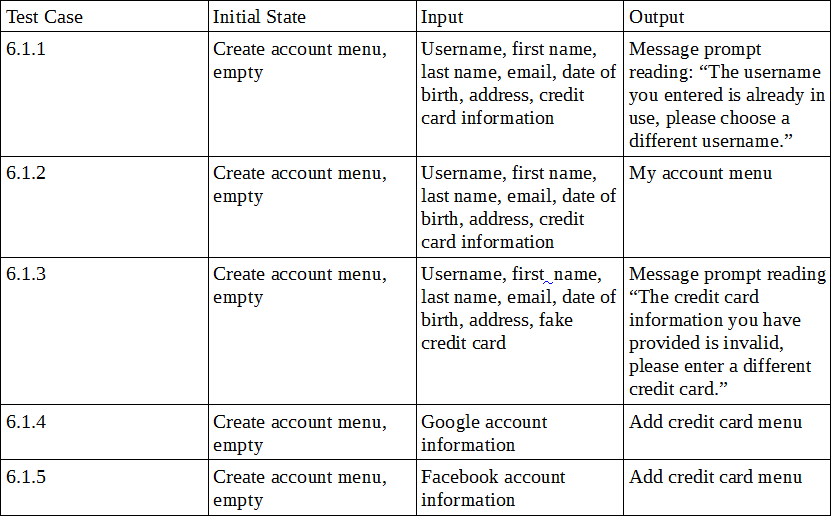
\includegraphics[width=\textwidth,height=\textheight,keepaspectratio]{accountTC.png}


\subsection{Order Transaction}
Smart-Waiter needs to ensure that a user can send in their order, and pay for their order easily and securely. Order transaction will be vigorously tested to ensure complete customer satisfaction.  
\subsubsection{Test Type}
Manual, functional dynamic test 
\subsubsection{Test Factors}
Correctness, reliability, data integrity, data security, ease of use

\begin{comment}
\subsubsection{Inputs}
A set \texorpdfstring{n\textsubscript{i}}{ni} of 10 random orders consisting of different menu items, created manually, where i = 0, 1, 2 .. 9, where i = 0..4 are invalid orders with respect to the restaurant's policies and where i = 5..9 are valid orders. \\
A valid credit card \\
An expired credit card \\
A fake credit card \\
A VISA debit card \\
A VISA gift card \\
\subsubsection{Outputs}
An order summary \texorpdfstring{O\textsubscript{i}}{Oi}, where i corresponds to the \texorpdfstring{i\textsuperscript{th}}{ith} order from the set of orders \texorpdfstring{n\textsubscript{i}}{ni}. \\
A message M, containing either a success or failure message, depending on the card type used. 
\end{comment}

\subsubsection{Initial State}
Order Test Cases: Restaurant menu module
Credit Card Test Cases: Payment confirmation menu
\subsubsection{Methods of testing}
Dynamic testing is used to ensure validity, record the number of successful tests given a sample.
\subsubsection{Test Cases}
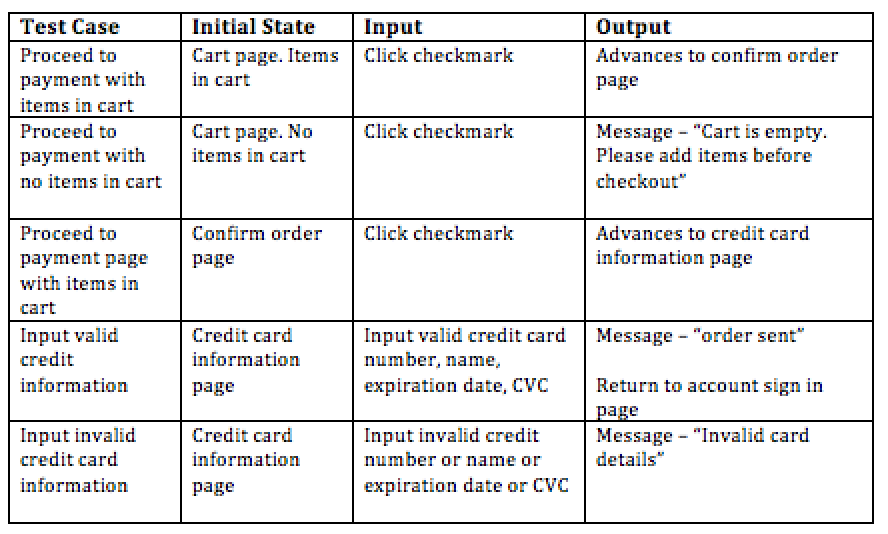
\includegraphics[width=\textwidth,height=\textheight,keepaspectratio]{orderTransactionTC.png}

\subsection{Usability Testing}
The goal of usability testing is to verify if a user can successfully use all functionalities of the application from start to finish in a timely manner. This type of testing aids in evaluating if functional requirements are met. As well it provides scope for evaluating non functional requirements.
\subsubsection{Test Factors}
\begin{itemize}
  \item Reliability 
  \item Performance
  \item 	Correctness
  \item 	Ease of use
\end{itemize}
\subsubsection{Inputs}
Input will consist of user input for entire app:
\begin{itemize}
  \item Account login
  \item Barcode
  \item Menu items selected
  \item Credit card details
\end{itemize}
\subsubsection{Outputs}
Output will consist of a response for each user input:
\begin{itemize}
  \item Successful login in response to account login
  \item Restaurant menu in response to barcode scan
  \item Order confirmation in response to menu items selected
  \item Transaction confirmation in response to credit card transaction
\end{itemize}
\subsubsection{Initial State}
\begin{itemize}
  \item User starts at the beginning of the process; account login page
\end{itemize}
\subsubsection{Methods of testing}
\begin{itemize}
  \item Functional unit test
\end{itemize}
\subsubsection{Test Cases}
\textbf{\textit{Functional Unit Test}}\newline
\newline
\textit{Summary}\newline
Manual black box tests will be performed to assess usability of the application. This test will be in the form of unit testing. Ten participants will be selected to evaluate this test. At least five will have some experience with using android applications. The remaining will have little to no experience. Each participant will be asked to conduct a walk through of the application. Number of errors made will be counted and recorded to further evaluate functional requirements and improve test cases. As well, qualitative feedback from participants will be taken in the end. For example, participants will be asked to comment on things they liked and things they didn't like. Also, they will be asked to provide a rating out of 10 in terms of experience; 1 being a poor experience and 10 being a wonderful experience. This feedback will help evaluate non function requirements; user interface appearance, learning requirements and accessibility. 
\newline

\section{Automated Testing Plan}


\end{document}
